\section{Related Work}
\label{sec:related_work}

\begin{figure*}[htbp]
    \centering
    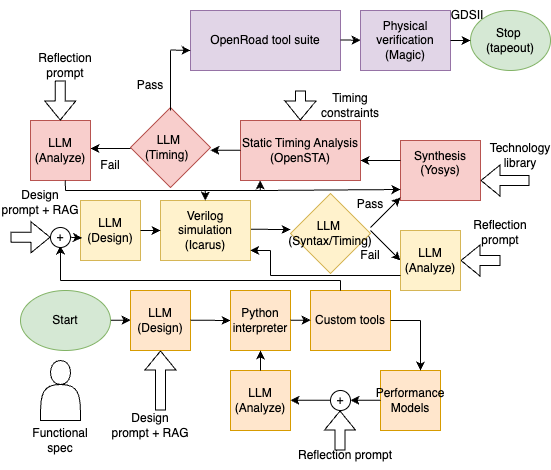
\includegraphics[width=0.6\textwidth]{figs/system_design_v2.png} 
    \caption{Proposed agentic AI design framework for digital ASIC design. The design flow is broadly divided into four parts: 1) Architecture design (shaded orange), 2) RTL design (shaded yellow), 3) Netlist synthesis (shaded red), and 4) Physical design (shaded purple). At each stage, the design is driven by a combination of LLM and appropriate EDA tools operating in a feedback loop.  }
    \label{fig:agentic_designflow}
\end{figure*}
We review previous reported work on the use of Generative AI in chip design. DAVE \cite{dave} and Verigen \cite{verigen} were among the first works to exploit the use of LLMs in HDL generation. Their focus is on improving LLM performance by fine-tuning the open source LLM models for Verilog code generation. 

The ChipNemo project \cite{chipnemo} from Nvidia does not directly target the use of LLMs in the design of digital systems. Instead, domain-specific LLMs are designed for supporting ancillary tasks such as a chatbot that serves as an engineering assistant, EDA script generation, and bug summarization and analysis. Their efforts are thus complementary to our proposed work. 

Recognizing the need to augment and fine-tune LLMs for hardware design, the MG-Verilog \cite{mg-verilog} project proposes an open source dataset consisting of over 11,000 Verilog code samples and their corresponding natural language descriptions. MG-Verilog dataset is complementary to our effort, and could be used to make the underlying foundational models more accurate through techniques such as Retrieval Augmented Generation (RAG), and fine tuning.  

In the GPT4AIChip project \cite{gpt4aigchip}, a feedback design loop is proposed consisting of prompting the LLM with human-crafted design examples (few-shot learning) and an evolutionary algorithm-based design space exploration algorithm to explore the designs generated by the LLM.  The LLM generated code for a matrix multiplier (GEMM) for is synthesized and evaluated on an FPGA using the Xilinx Vivado HLS tools. The design flow proposed by GPT4AIChip can be considered agentic, but its design exploration space is constrained. In contrast to our approach, it does not address the more complex ASIC design flow, including synthesis, and timing analysis.

The AutoChip \cite{autochip} project proposes an automated approach that uses large language models (LLMs) to generate HDL. AutoChip combines conversational LLMs such as OpenAI GPT-4 with feedback from Verilog compilers and simulations to iteratively improve Verilog modules. Starting with an initial module generated from a design prompt, it refines the design based on errors and simulation messages. AutoChip's effectiveness is evaluated using design prompts and test benches from HDLBits, a collection of small circuit design exercises. Although AutoChip uses an agent-based design flow, unlike our system's design focus, it is limited to small circuits and lacks a comprehensive end-to-end design flow.

 
